\section*{Abstract}
\addcontentsline{toc}{section}{Abstract}
This report studies next-day market-movement classification (\emph{Fall}, \emph{Neutral}, \emph{Rise}) on the public \textbf{NIFTY} benchmark (SPY, 2010--2020) using lagged market data, financial news headlines encoded by a frozen \textbf{FinBERT} model, and data-driven \textbf{market regimes} obtained by clustering rolling return and volatility. Two questions are asked: \emph{how sensitive is reported performance to the evaluation protocol}, and \emph{do news and regime information add predictive value beyond lagged prices}, in particular across volatility regimes and during the February--April 2020 stress period.

A small family of models (price-only, price plus news, price plus news plus regime, and ablations) is trained with fixed hyper-parameters, ten random seeds and three protocols: a random split, a chronological split with preprocessing fitted on all data, and a strict chronological split with train-only preprocessing. Under the strict protocol all models beat a random-guess floor (Macro-F1 $0.333$), but a price-only LSTM ($0.466$) was \emph{not} improved by 768-dimensional FinBERT embeddings ($0.416$, a statistically reliable decrease), by three FinBERT sentiment scores ($0.482$, difference $+0.016$ with an interval containing zero) or by an explicit regime input. Relaxing the protocol produced no systematic optimism, except for a model that uses only the persistent regime label. A data audit also showed that the benchmark label is the \emph{next} trading day's return and that a daily price series can be recovered from the supplied contexts. The study is a methodological analysis, not a trading system.

\begin{figure}[H]
\centering
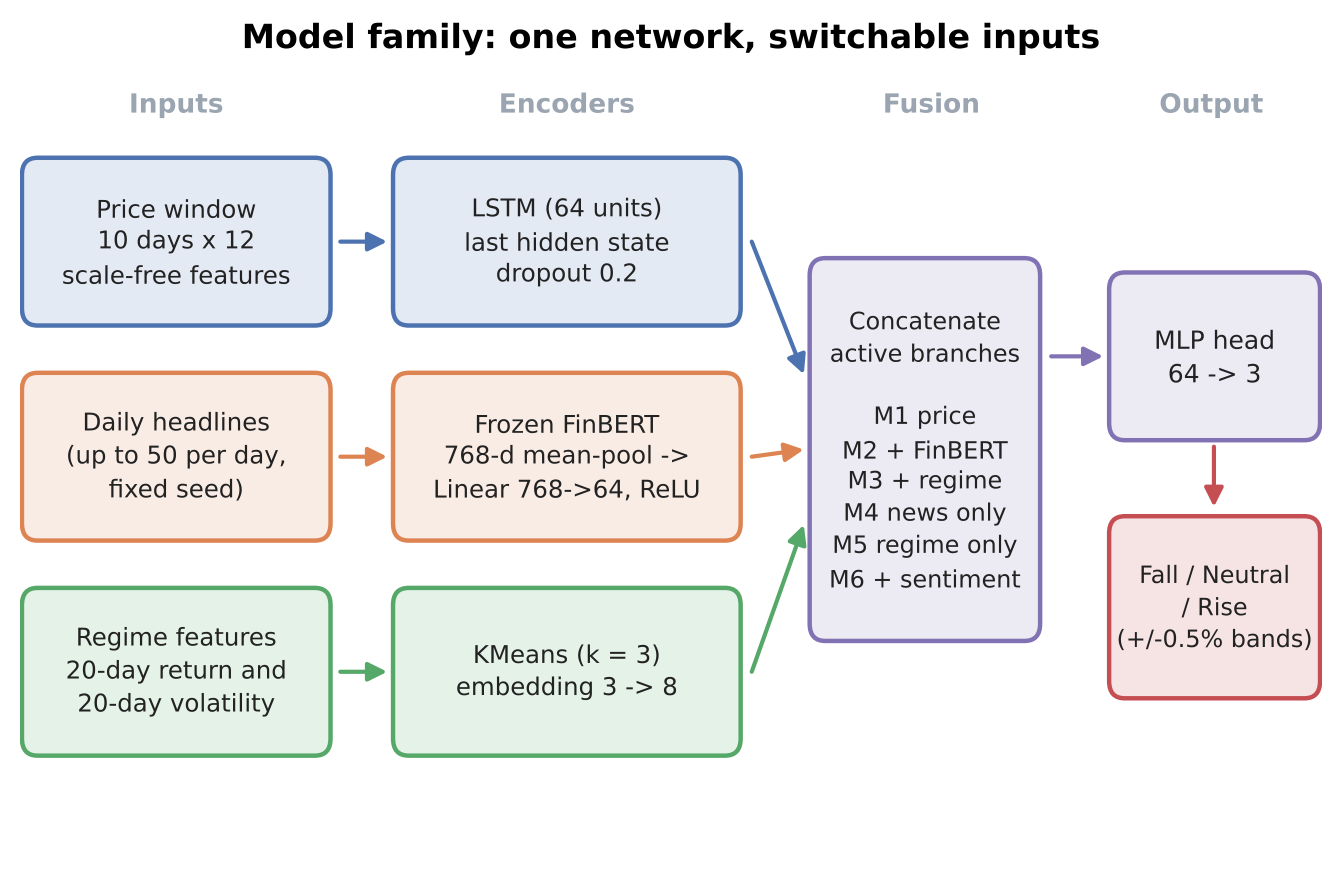
\includegraphics[width=0.96\textwidth]{fig_architecture.png}
\caption{Model family used in this report: one small network with switchable information sources.}
\end{figure}
